\section{Introduction}
\label{sec:intro}

Suppose a valve has four positions and its pointer last showed position zero.
After a clockwise turn the valve is at position one. If the turn goes
unrecorded, however, the valve could be at zero, one, or three, and a controller
must decide whether to act on its current estimate or pay to read the pointer
again. The same problem arises whenever a state moves around a known cycle,
whether it is a valve setting or the heading of a moving sensor. We write $\Z_k$
for a cycle of $k$ positions, numbered from $0$ to $k-1$ with wraparound
\citep{kaelbling1998pomdp}.

What a model has to do depends on how the position is observed. If every turn is
visible, the model only needs to carry the count forward. If a sensor gives only
a noisy cue, the model must first infer which turn occurred. If the cue is
missing altogether, the model has to keep a probability for each possible
position; we call this distribution the \emph{belief}. Figure~\ref{fig:overview}
illustrates the first two cases and the two structures we compare.

\begin{figure}[!htbp]
\centering
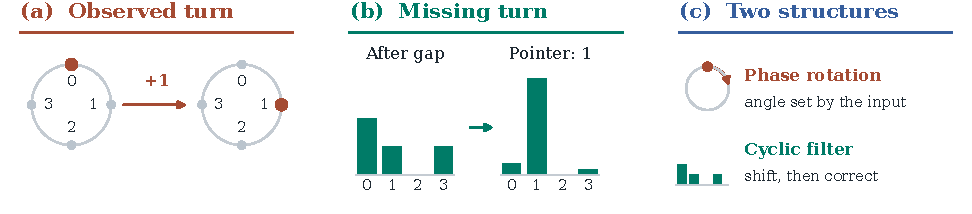
\includegraphics[width=\linewidth]{figures/overview_tracking.pdf}
\caption{From observations to actions in a four-position cycle.
(a) An observed turn moves the valve from position 0 to 1.
(b) An unrecorded turn leaves several possible positions. The bars show the
probability of each position before and after a noisy pointer reading of 1.
(c) The two structures we study: a phase rotation with its angle set by the
input, and a cyclic filter that shifts a belief and corrects it with a reading.}
\label{fig:overview}
\label{fig:method}
\end{figure}

This paper asks where a known cycle should enter a learned model.
Section~\ref{sec:method} describes two options. A \emph{phase rotation} builds the
cycle into the state update: the input sets a rotation angle, and a
squared-amplitude readout turns the rotated state into probabilities. A
\emph{cyclic filter} builds the cycle into the belief update instead: it shifts a
distribution over positions and then corrects it with a pointer reading.
Section~\ref{sec:exp} compares both structures with recurrent and attention
models in simulation, as the observations degrade from clean to noisy to
missing. To see whether a better belief also leads to better decisions, we give
every estimator's belief to the same planner. Beliefs are scored by the negative
log likelihood (NLL) of the true position, and control by net utility, the
success indicator minus the cost of turns and readings. Section~\ref{sec:imu}
then tests both structures on a recorded inertial sensor.

The answer depends on where the uncertainty enters. With clean events, letting
the input set the rotation angle is what allows a policy to learn the count from
a terminal reward. With noisy or missing events, the cyclic filters give the most
accurate beliefs, although a shared planner turns these better beliefs into
only small gains in net utility; the clearest effect is on whether the planner
takes another reading. On the recorded sensor, a rotation driven by the measured
gyroscope increment stays accurate far beyond its training length, whereas
recurrent and attention models given the same inputs do not. A classical filter
with bias estimation remains more accurate than all learned models.

\subsection{Related work}
\label{sec:related}

\myparagraph{Representing a cyclic state.}
Unitary RNNs and oscillatory recurrences use norm-preserving or undamped
dynamics \citep{arjovsky2016urnn,rusch2021cornn}. \citet{grazzi2025negative} give
an exact two-coordinate rotation and a linear template decoder for modular
counting. Our phase rotation uses the same input-dependent rotation as the
cyclic construction of \citet{karuvally2025aussm}, and
\citet{shakerinava2026diagonal} characterize the broader Abelian case for complex
diagonal state-space models. DeltaProduct tracks groups and extrapolates in
length through products of Householder updates \citep{siems2025deltaproduct}. We
use a small official-layer adapter, and its results apply to the tested width,
depth, and training recipe.

\myparagraph{Counting on longer sequences.}
Parity and modular counting are standard probes of length extrapolation
\citep{deletang2023chomsky}. Transformers can fit these tasks through
length-specific shortcuts \citep{liu2023shortcuts,zhou2024rasp}, and state-space
models and Transformers face expressivity limits on group word problems
\citep{merrill2024illusion}. Networks trained on modular arithmetic discover
Fourier features \citep{nanda2023grokking,chughtai2023universality,zhong2023clock},
and residue hyperdimensional computing combines unit-root codes by phasor
multiplication \citep{kymn2025residue}. We ask a different question: whether a model
can learn to count from a terminal reward, and how the answer changes when events
are noisy or missing.

\myparagraph{Memory and belief under partial observation.}
Recurrent policies are a standard baseline
\citep{hausknecht2015drqn,ni2022recurrent}. Reward machines provide automaton
memory learned from experience \citep{icarte2019reward}. Hidden actions and
occasional state reveals have been studied with probabilistic automata
\citep{siems2026code}. \citet{zhao2026belief} relate recurrent memory to belief
logits under deterministic transitions and extend their filters to
action-controlled settings. Born probabilities have also been used to
parameterize quantum-circuit policies \citep{jerbi2021parametrized}; our readout
is a classical squared amplitude. Unlike these works, we isolate the effect of a
belief on decisions by giving every estimate to the same planner.

\myparagraph{Inertial heading estimation.}
Complementary filters fuse gyroscope integration with gravity and magnetic
references \citep{mahony2008complementary}. VQF adds gyroscope bias estimation
and magnetic disturbance rejection \citep{laidig2023vqf}, and the BROAD benchmark
records these conditions with an optical reference \citep{laidig2021broad}. We
report both filters alongside the learned models.
